\chapter{Vision, Language, and Logic: Robustness to Logical Compositions}
\label{chap:vqalol}

%%%%%%%%%%%%%%%%%%%%%%%%%%%%%%%%%%%%%%%%%%%%%%%%%%%%%%%%%%%%%%%%
% \begin{abstract}
%%%%%%%%%%%%%%%%%%%%%%%%%%%%%%%%%%%%%%%%%%%%%%%%%%%%%%%%%%%%%%%%
Logical connectives and their implications on the meaning of a natural language sentence are a fundamental aspect of understanding.
In this paper, we investigate whether visual question answering (VQA) systems trained to answer a question about an image, are able to answer the logical composition of multiple such questions.
When put under this \textit{Lens of Logic}, state-of-the-art VQA models have difficulty in correctly answering these logically composed questions.
We construct an augmentation of the VQA dataset as a benchmark, with questions containing logical compositions and linguistic transformations (negation, disjunction, conjunction, and antonyms).
We propose our {Lens of Logic (LOL)} model which uses question-attention and logic-attention to understand logical connectives in the question, and a novel Fréchet-Compatibility Loss, which ensures that the answers of the component questions and the composed question are consistent with the inferred logical operation.
Our model shows substantial improvement in learning logical compositions while retaining performance on VQA.
We suggest this work as a move towards robustness by embedding logical connectives in visual understanding.
% \end{abstract}

\begin{figure}
    \centering
    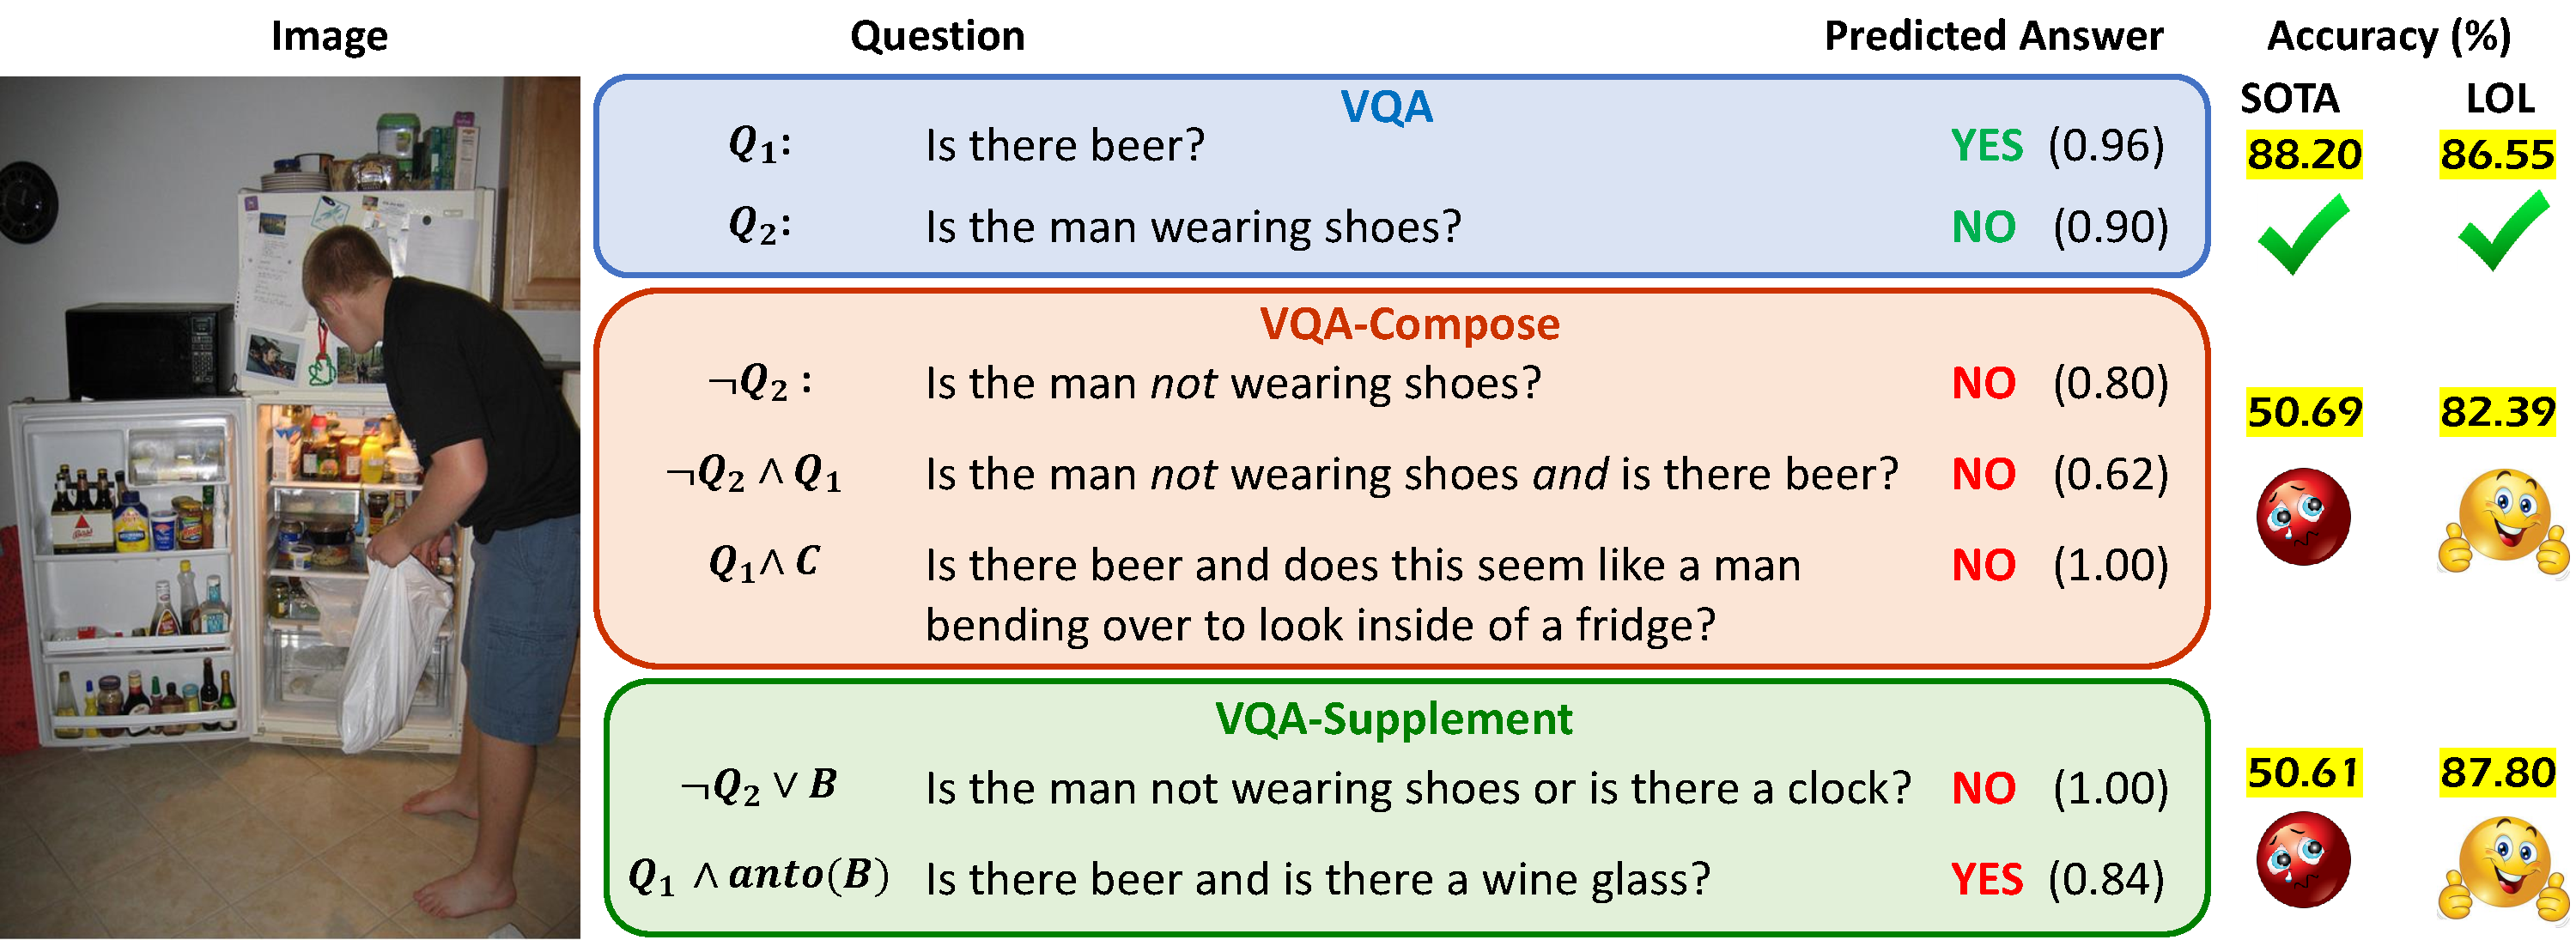
\includegraphics[width=\linewidth]{vqalol/images/teaser_final.pdf}
    \caption{
        % Illustration of logical composition of questions. 
        State-of-the-art models answer questions from the VQA dataset ($Q_1, Q_2$) correctly, but struggle when asked a logical composition including negation, conjunction, disjunction, and antonyms. 
        We develop a model that improves on this metric substantially, while retaining VQA performance.
        }
    \label{fig:motivation}
\end{figure}%
%%%%%%%%%%%%%%%%%%%%%%%%%%%%%%%%%%%%%%%%%%%%%%%%%%%%%%%%%%%%%%%%
\section{Introduction}
%%%%%%%%%%%%%%%%%%%%%%%%%%%%%%%%%%%%%%%%%%%%%%%%%%%%%%%%%%%%%%%%
Theories about logic in human understanding have a long history. 
In modern times, Piaget and Fodor~\citep{piattelli1980language} studied the representation of logical hypotheses in the human mind.
George Boole~\citep{boole1854investigation} formalized conjunction, disjunction, and negation into an ``algebra of thought'' as a way to improve, systemize, and mathematize Aristotle's Logic~\citep{corcoran1972completeness}.
Horn regarded negation to be a fundamental and defining characteristic of human communication~\citep{horn2000negation}, following the traditions of Sankara~\citep{raju1954principle}, Spinoza~\citep{spinoza1934ethics}, and Hegel~\citep{hegel1929hegel}.
Recent studies~\citep{arlotti1263} have suggested that infants can formulate intuitive and stable logical structures to interpret dynamic scenes and to entertain and rationally modify hypotheses about the scenes.
As such we argue that understanding logical structures in questions, is a fundamental requirement for any question-answering system.
\begin{quotation}
    \begin{quote}
        \textit{If a question can be put at all, then it can be answered.}\\\hspace*{\fill}{\citet{wittgenstein2013tractatus}}
    \end{quote}
\end{quotation}
In the above proposition, Wittgenstein linked the process of asking a question with the existence of an answer.
While we do not comment on the existence of an answer, we suggest the following softer proposition -
\begin{quotation}
    \begin{quote}
        \textit{If questions $Q_1\dots Q_n$ can be answered, then so should all composite questions created from $Q_1\dots Q_n$}
    \end{quote}
\end{quotation}

Visual question answering (VQA)~\citep{antol2015vqa} is an intuitive, yet challenging task that lies at a crucial intersection of vision and language. 
Given an image and a question about it, the goal of a VQA system is to provide a free-form or open-ended answer.
Consider the image in Figure~\ref{fig:motivation} which shows a person in front of an open fridge.
When asked the questions $Q_1$ ({\it Is there beer?}) and $Q_2$ ({\it Is the man wearing shoes?}) independently, the state-of-the-art model LXMERT~\citep{tan2019lxmert} answers both correctly.
However when we insert a negation in $Q_2$ ({\it Is the man not wearing shoes?}) or for a conjunction of two questions $\neg Q_2 \wedge Q1$ ({\it Is the man not wearing shoes and is there beer?}), the system makes wrong predictions. 
Our motivation is to reliably answer such logically composed questions.
In this paper, we analyze VQA systems under this {\it Lens of Logic (LOL)} and develop a model that can answer such questions reflecting human logical inference.
We offer our work as the first investigation into the logical structure of questions in visual question-answering and provide a solution that {\it learns} to interpret logical connectives in questions.

The first question is: can models pre-trained on the VQA dataset answer logically composed questions?
It turns out that these models are unable to do so, as illustrated in Figure~\ref{fig:motivation} and Table~\ref{table:exp1}.
An obvious next experiment is to \textit{split the question} into its component questions, predict the answer to each, and combine the answers logically. 
However language parsers (either oracle or trained parsers) are not accurate at understanding negation, and as such this approach does not yield correct answers for logically composed questions.
The question then arises: can the model answer such questions, if we explicitly train it with data that also contains logically composed questions?
For this investigation, we construct two datasets, \texttt{VQA-Compose} and \texttt{VQA-Supplement}, by utilizing annotations from the VQA dataset, as well as object and caption annotations from COCO~\citep{lin2014microsoft}.
We use these datasets to train the state-of-the-art model LXMERT~\citep{tan2019lxmert} and perform multiple experiments to test for robustness towards logically composed questions.

After this investigation, we develop our LOL model architecture that jointly learns to answer questions while understanding the type of question and which logical connective exists in the question, through our attention modules, as shown in Figure~\ref{fig:model}.
We further train our model with a novel Fréchet-Compatibility loss that ensures compatibility between the answers to the component questions and the answer of the logically composed question.
One key finding is that our models are better than existing models trained on logical questions, with a small deviation from state-of-the-art on VQA test set.
Our models also exhibit better {\it Compositional Generalization} i.e. models trained to answer questions with a single logical connective are able to answer those with multiple connectives.

Our contributions are summarized below:
\begin{enumerate}[noitemsep]
    \item We conduct a detailed analysis of the performance of the state-of-the-art VQA model with respect to logically composed questions,
    \item We curate two large scale datasets \texttt{VQA-Compose} and \texttt{VQA-Supplement} that contain logically composed binary questions.
    \item We propose \textit{LOL} -- our end-to-end model with dedicated attention modules that answer questions by understanding the logical connectives in questions.
    \item We show a capability of answering logically composed questions, while retaining VQA performance. % on VQA data.
\end{enumerate}

%%%%%%%%%%%%%%%%%%%%%%%%%%%%%%%%%%%%%%%%%%%%%%%%%%%%%%%%%%%%%%%%
\section{Related Work}
%%%%%%%%%%%%%%%%%%%%%%%%%%%%%%%%%%%%%%%%%%%%%%%%%%%%%%%%%%%%%%%%
\noindent\textbf{Logic in Human Expression:}
Is logical thinking a natural feature of human thought and expression?
Evidence in psychological studies~\citep{carey1985conceptual,gopnik1999scientist,arlotti1263} suggests that infants are capable of logical reasoning, toddlers understand logical operations in natural language and are able to compositionally compute meanings even in complex sentences containing multiple logical operators.
Children are also able to use these meanings to assign truth values to complex experimental tasks.
Given this, question-answering systems also need to answer compositional questions, and be robust to the manifestation of logical operators in natural language.\\

\noindent\textbf{Logic in Natural Language Understanding:}
The task of understanding compositionality in question-answering (QA) can also be interpreted as understanding logical connectives in text.
While question compositionality is largely unstudied, approaches in natural language understanding seek to transform sentences into symbolic formats such as first-order logic (FOL) or relational tables~\citep{mintz2009distant,zettlemoyer2012learning,lewis-steedman-2013-combined}.
While such methods benefit from interpretability, they suffer from practical limitations like intractability, reliance on background knowledge, and failure to process noise and uncertainty. 
\citep{bordes2013translating,riedel-etal-2013-relation,socher2013reasoning} suggest that better generalization can be achieved by learning embeddings to reason about semantic relations, and to simulate FOL behavior~\citep{rocktaschel2014low}.
Recursive neural networks have been shown to learn logical semantics on synthetic English-like sentences by using embeddings~\citep{bowman2014recursive,neelakantan2015compositional}.

Detection of negation in text has been studied for information extraction and sentiment analysis~\citep{morante2012modality}.
\citep{kassner2019negated} have shown that BERT-based models~\citep{devlin2018bert,liu2019roberta} are incapable of differentiating between sentences and their negations.
Concurrent to our work,~\citep{asai-hajishirzi-2020-logic} show the efficacy of FOL-guided data augmentation for performance improvements on natural language QA tasks that require reasoning.
Since our work deals with both vision and language modalities, it encounters a greater degree of ambiguity, thus calling for robust VQA systems that can deal with logical transformations.\\

\noindent\textbf{Visual Question Answering}
(VQA)~\citep{antol2015vqa} is a large-scale, human-annotated dataset for open-ended question-answering on images.
VQA-v2\citep{goyal2017making} reduces the language bias in the dataset by collecting complementary images for each question-image pair.
This ensures that the number of questions in the VQA dataset with the answer ``YES" is equal to those with the answer ``NO".
This dataset contains 204k images from MS-COCO~\citep{lin2014microsoft}, and 1.1M questions.

Cross-modal pre-trained models ~\citep{tan2019lxmert,lu2019vilbert,zhou2020unified} have proved to be highly effective in vision-and-language tasks such as VQA, referring expression comprehension, and image retrieval. 
While neuro-symbolic approaches~\citep{Mao2019NeuroSymbolic} have been proposed for VQA tasks which require reasoning on synthetic images, their performance on natural images is lacking.
Recent work seeks to incorporate reasoning in VQA, such as visual commonsense reasoning~\citep{zellers2019recognition,fang2020video2commonsense}, spatial reasoning~\citep{hudson2019gqa,johnson2017clevr}, and by integrating knowledge for end-to-end reasoning~\citep{Aditya:2019:IKR:3367722.3367926}.

We take a step back and extensively analyze the pivotal task of VQA with respect to various aspects of generalization.
We consider a rigorous investigation of a task, dataset, and models to be equally important as proposing new challenges that are arguably harder.
In this paper we analyse existing state-of-the-art VQA models with respect to their robustness to logical transformations of questions.

%%%%%%%%%%%%%%%%%%%%%%%%%%%%%%%%%%%%%%%%%%%%%%%%%%%%%%%%%%%%%%%%
\section{The Lens of Logic}
%%%%%%%%%%%%%%%%%%%%%%%%%%%%%%%%%%%%%%%%%%%%%%%%%%%%%%%%%%%%%%%%
\begin{table}[!t]
    \centering
    \begin{tabular}{@{}lp{8.6cm}lc@{}}
    \toprule 
    \textbf{QF} & \textbf{Question} & \textbf{AF} & \textbf{Answer}\\
    \midrule
    $Q_1$                       & Is there beer?                                    & $A_1$     & Yes \\
    $Q_2$                       & Is the man wearing shoes?                         & $A_2$     & No \\
    ${\neg}Q_1$                  & Is there no beer?                                 & ${\neg}A_1$ & No\\
    ${\neg}Q_2$                  & Is the man not wearing shoes?                     & ${\neg}A_2$ & Yes\\
    $Q_1{\wedge}Q_2$            & Is there beer and is the man wearing shoes?       & $A_1{\wedge}A_2$ & No \\
    $Q_1{\vee}Q_2$              & Is there beer or is the man wearing shoes?        & $A_1{\vee}A_2$ & Yes \\
    $Q_1{\wedge}{\neg}Q_2$       & Is there beer and is the man not wearing shoes?   & $A_1{\wedge}{\neg}A_2$ & Yes \\
    $Q_1{\vee}{\neg}Q_2$         & Is there beer or is the man not wearing shoes?    & $A_1{\vee}{\neg}A_2$ & Yes \\
    ${\neg}Q_1{\wedge}Q_2$       & Is there no beer and is the man wearing shoes?    & ${\neg}A_1{\wedge}A_2$ & No \\
    ${\neg}Q_1{\vee}Q_2$         & Is there no beer or is the man wearing shoes?     & ${\neg}A_1{\vee}A_2$ & No \\
    ${\neg}Q_1{\wedge}{\neg}Q_2$  & Is there no beer and is the man not wearing shoes?& ${\neg}A_1{\wedge}{\neg}A_2 $ & No \\
    ${\neg}Q_1{\vee}{\neg}Q_2$    & Is there no beer or is the man not wearing shoes? & ${\neg}A_1{\vee}{\neg}A_2$ & Yes \\
    \bottomrule
    \end{tabular}
    \caption{Illustration of question composition in \texttt{VQA-Compose}, for the same example as in Figure \ref{fig:motivation}.
    QF: Question Formula, AF: Answer Formula}
    \label{tab:compose}
\end{table}

\begin{figure}[t]
    \centering
    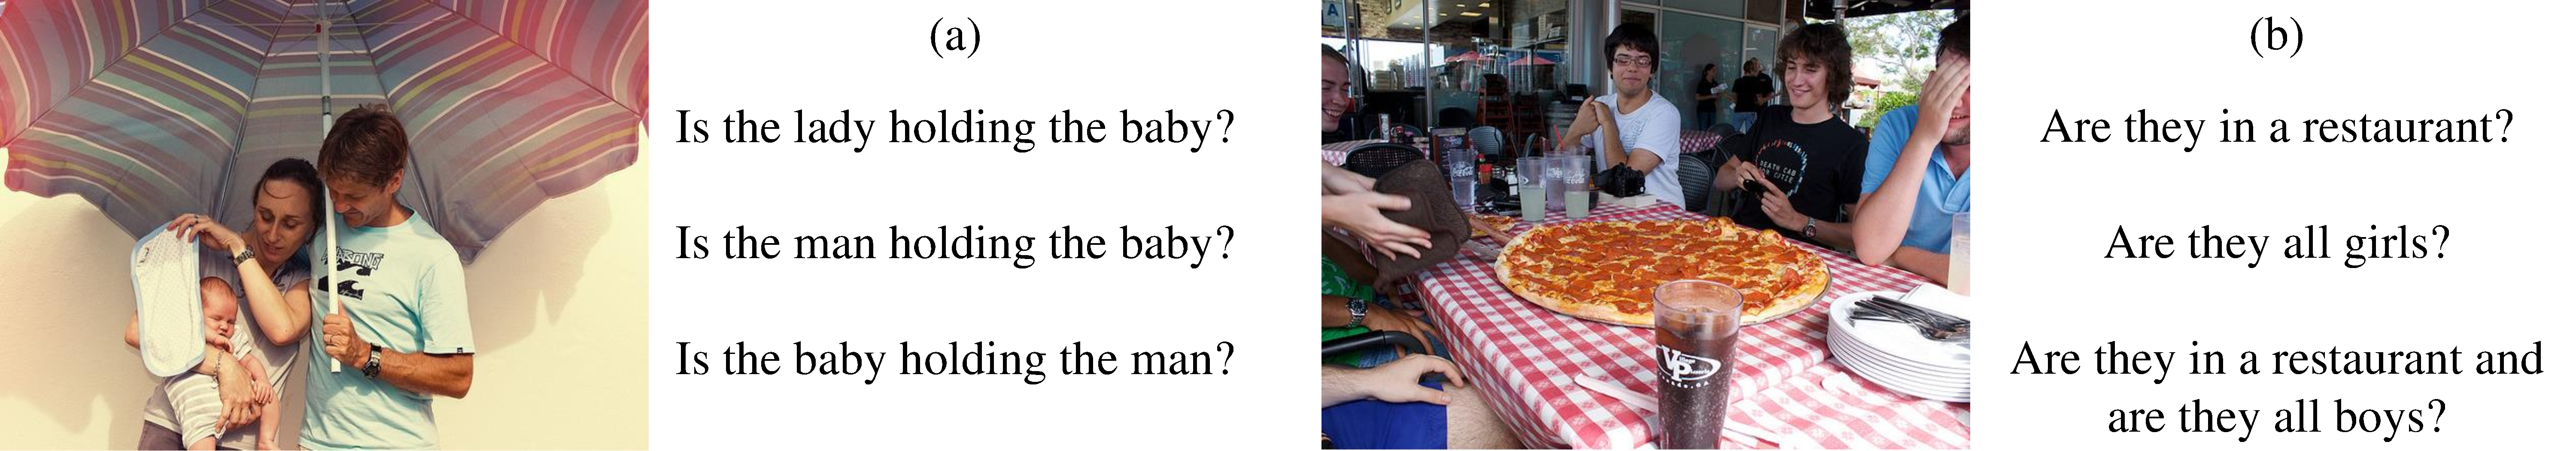
\includegraphics[width=\linewidth]{vqalol/images/illus.pdf}
    \caption{Some questions in \texttt{VQA-Supplement} created with adversarial antonyms.}
    \label{fig:illus}
\end{figure}

A lens magnifies objects under investigation, by allowing us to zoom and focus on desired contents or processes.
Our lens of logical composition of questions, allows us to magnify, identify, and analyze the problems in VQA models.

Consider Figure~\ref{fig:illus}(a), where we transform the first question {\it ``Is the lady holding the baby"} by first replacing {\it ``lady"} with an adversarial antonym {\it ``man"} and observe that the system provides a wrong answer with very high probability.
Swapping {\it ``man"} with {\it ``baby"} results in a wrong answer as well.
In~\ref{fig:illus}(b) a conjunction of two questions containing antonyms ({\it girls} vs {\it boys}) yields a wrong answer.
We identify that the ability to answer composite questions created by negation, conjunction and disjunction of questions is crucial for VQA.

We use ``closed questions" as defined in~\citep{bobrow1964natural} to construct logically composed questions. 
Under this definition, if a closed question has a negative (``NO") answer then its negation must have an affirmative (``YES") answer.
Of the three types of questions in the VQA dataset (yes/no, numeric, other), `yes-no" questions satisfy this requirement.
Although, visual questions in the VQA dataset can have multiple correct answers~\citep{bhattacharya2019does}, $20.91\%$ of the questions (around 160k) in the VQA dataset are closed questions, i.e. questions with a single unambiguous yes-or-no answer, unanimously annotated by multiple human workers.
This allows us to treat these questions as propositions and create a truth table for answers to compose logical questions as shown in Table~\ref{tab:compose}.

    \subsection{Composite Questions}
    Let $\mathcal{D}$ be the VQA dataset. 
    For closed questions $Q_1$ and $Q_2$ about image $I\in\mathcal{D}$, we define the composite question $Q^*$ composed using connective $\circ\in\{ \vee, \wedge\}$, as:
    \begin{equation}
        Q^* = \widehat{Q_1} ~\circ ~\widehat{Q_2}, \qquad where~~ \widehat{Q_1} \in \{ Q_1, \neg Q_1\},  ~ \widehat{Q_2} \in \{ Q_2, \neg Q_2\}. 
    \end{equation}
    
    \subsection{Dataset Creation Process}
    Using the above definition we create two new datasets by utilizing multiple questions about the same image (\texttt{VQA-Compose}) and external object and caption annotations about the image from COCO to create more questions (\texttt{VQA-Supplement}).
    The seed questions for creating these datasets are all closed binary questions from VQA-v2~\citep{goyal2017making}.
    These datasets serve as test-beds, and enable experiments that analyze performance of models when answering such questions.\\

        \noindent\textbf{VQA-Compose:}
        Consider the first two rows in Table~\ref{tab:compose}. 
        $Q_1$ and $Q_2$ are two questions about the image in Figure~\ref{fig:motivation} taken from the VQA dataset.
        Additional questions are composed from $Q_1$ and $Q_2$ by using the formulas in Table~\ref{tab:compose}.
        Thus for each pair of closed questions in the VQA dataset, we get 10 logically composed questions.
        Using the same train-val-test split as the VQA-v2 dataset~\citep{goyal2017making}, we get \textit{1.25 million samples} for our \texttt{VQA-Compose} dataset.
        The dataset is balanced in terms of the number of questions with affirmative and negative answers.\\
        
        \noindent\textbf{VQA-Supplement:}
        Images in VQA-v2 follow identical train-val-test splits as their source MS-COCO~\citep{lin2014microsoft}.
        Therefore, we use the object annotations from COCO to create additional closed binary questions, such as {\it ``Is there a bottle"} for the example in Figure~\ref{fig:motivation}.
        We also create ``adversarial" questions about objects, like {\it ``Is there a wine-glass?"} by using an object that is not present in the image (wine-glass), but is \textit{semantically close} to an object in the image (bottle).
        We use Glove vectors~\citep{pennington2014glove} to find the adversarial object with the closest embedding. 
        Following a similar strategy, we also convert captions provided in COCO to closed binary questions, for example {\it ``Does this seem like a man bending over to look inside the fridge"}.
        Since we know what objects are present in the image, and the captions describe a ``true" scene, we are able to obtain the ground-truth answers for questions created from objects and captions.
        Similar methods for creation of question-answer pairs have previously been used in~\citep{ren2015exploring,malinowski2014multi}.

        Thus for every question, we obtain several questions from objects and captions, and use these to compose additional questions by following a process similar to the one for \texttt{VQA-Compose}.
        For each closed question in the VQA dataset, we get $20$ additional logically composed questions by utilizing questions created from objects and captions, yielding a total of \textit{2.55 million samples} as \texttt{VQA-Supplement}.

    \subsection{Analytical Setup}
    In order to test the robustness of our models to logically composed questions, we devise five key experiments to analyse baseline models and our methods.
    These experiments help us gain insights into the nuances of the VQA dataset, and allow us to develop strategies for promoting robustness.\\

        \noindent\textbf{Effect of Data Augmentation:}
        In this experiment, we compare the performance of models on \texttt{VQA-Compose} and \texttt{VQA-Supplement} with or without logically composed training data.
        This experiment allows us to test our hypotheses about the robustness of any VQA model to logically composed questions.
        We first use models trained on VQA data to answer questions in our new datasets and record performance.
        We then explicitly train the same models with our new datasets, and make a comparison of performance with the pre-trained baseline.\\
        
        \noindent\textbf{Learning Curve:}
        We train our models with an increasing number of logically composed questions and compare performance.
        This serves as an analysis of the number of logical samples needed by the model to understand logic in questions.\\
    
        \noindent\textbf{Training only with Closed Questions:}
        In this ablation study, we restrict the training data to only closed questions i.e. ``Yes-No" VQA questions, \texttt{VQA-Compose} and \texttt{VQA-Supplement}, allowing our model to focus solely on closed questions.\\
    
        \noindent\textbf{Compositional Generalization:}
        We address whether training on closed questions containing single logical operation ($\neg Q_1$,  $Q_1\vee Q_2$) can generalize to multiple operations ($Q_1 \wedge \neg Q_2$, $\neg Q_1 \vee Q_2$).
        For instance, rows 1 through 6 in Table~\ref{tab:compose} are {\it single operation questions}, while rows 7 through 12 are {\it multi-operation questions}.
        Our aim is to have models that exhibit such compositional generalization.\\
        
        \noindent\textbf{Inductive Generalization:}
        We investigate if training on compositions of two questions ($\neg Q_1 \vee Q_2$) can generalize to compositions of more than two questions ($Q_1 \wedge \neg Q_2 \wedge Q_3 \dots$).
        This studies whether our models develop an understanding of logical connectives, as opposed to simply learning patterns from large data.

%%%%%%%%%%%%%%%%%%%%%%%%%%%%%%%%%%%%%%%%%%%%%%%%%%%%%%%%%%%%%%%%
\section{Method}
%%%%%%%%%%%%%%%%%%%%%%%%%%%%%%%%%%%%%%%%%%%%%%%%%%%%%%%%%%%%%%%%
\begin{figure}[t]
    \centering
    \includegraphics[width=\linewidth]{vqalol/images/vqa_lol_eccv.png}
    \caption{LOL model architecture showing a cross-modal feature encoder followed by our Question-Attention ($q_{\textit{\tiny ATT}}$) and Logic Attention ($\ell_{\textit{\tiny ATT}}$) modules. 
    The concatenated output of  is used by the Answering Module to predict the answer.
    % to the question (Q).
    }
    \label{fig:model}
\end{figure}

In this section. we describe LXMERT~\citep{tan2019lxmert} (a state-of-the-art VQA model), our Lens of Logic (LOL) model, attention modules which learn the question-type and logical connectives in the question, and the Fréchet-Compatibility (FC) Loss.
This section refers to a composition of two questions, but applies to $n\geq2$ questions.

    \subsection{Cross-Modal Feature Encoder}
    LXMERT (Learning Cross-Modality Encoder Representations from Transformers)~\citep{tan2019lxmert} is one of the first cross-modal pre-trained frameworks for vision-and-language tasks, that combines a strong visual feature extractor~\citep{ren2015faster} with a strong language model (BERT)\citep{devlin2018bert}.
    LXMERT is pre-trained for key vision-and-language tasks, on a large corpus of $\sim$9M image-sentence pairs, making it a powerful cross-modal encoder for vision+language tasks such as visual question answering, as compared to other models such as MCAN~\citep{Yu_2019_CVPR} and UpDn~\citep{Anderson2017up-down}, and strong representative baseline for our experiments.


    \subsection{Our Model: Lens of Logic (LOL)}
    The design for our LOL model is driven by three key insights:
    \begin{enumerate}[noitemsep]
        \item As logically composed questions are closed questions, understanding the type of question will guide the model to answer them correctly.
        \item Predicted answers must be compatible with the predicted question type. For instance, a closed question can have an answer that is either ``Yes" or ``No".
        \item The model must learn to identify the logical connectives in a question.
    \end{enumerate}

    \noindent Given these insights, we develop the Question Attention module that encodes the type of question (\textit{Yes-No}, \textit{Number}, or \textit{Other}), and the Logic Attention module that predicts the connectives (\textit{AND, OR, NOT, no connective}) present in the question, and use these to learn representations.
    The overall model architecture is shown in Figure~\ref{fig:model}.
    For every question $Q$ and corresponding image $I$, we obtain embeddings $z_Q$ and $z_I$ respectively, as well as a cross-modal embedding $z_X$. 

        \textbf{Question Attention Module ($q_{\textit{ATT}}$)}
        takes cross-modal embedding $z_x$ from LXMERT as input, and outputs vector \textbf{$P_{type} = softmax(\mathbf{q_{\textit{\tiny ATT}}}(z_x))$}, representing the probabilities of each question-type. 
        These probabilities are used to get a final representation $\mathbf{z^{type}}$ which combines the features for each question-type.\footnotemark[1]

        \textbf{Logic Attention Module ($\ell_{\textit{ATT}}$)}
        takes the cross-modal embedding $z_X$ from LXMERT as input, and outputs vector \textbf{$P^{conn} = \sigma(\mathbf{\ell_{\textit{ATT}}}(z_X))$} which represents the probabilities of each type of connective.
        We use sigmoid ($\sigma$) instead of a softmax, since a question can have multiple connectives.
        These probabilities are used to combine the features for each type of connective into a final representation $\mathbf{z^{conn}}$ which encodes information about the connectives in the question.

    \subsection{Loss Functions}
    We train our models jointly with the loss function given by:
    \begin{equation}
        \mathcal{L} = (1{-}\alpha_1{-}\alpha_2)\cdot \mathcal{L}_{ans} + \alpha_1 \cdot \mathcal{L}_{type} + \alpha_2 \cdot \mathcal{L}_{conn} + \beta\cdot\mathcal{L}_{\mathit{FC}}.
    \end{equation}

        \noindent\textbf{Answering Loss} $\ell_{ans}$ is conditioned on the type of question.
        We multiply the final prediction vector with the probability and the mask $M_i$ for question-type $i$.
        $M_i$ is a binary vector with $1$ for every answer-index of type-i and $0$ elsewhere:
        
        \begin{equation}
            \mathcal{L}_{\textit{ans}} = \mathcal{L}_{\textit{\tiny BCE}}(\sum_{i=1}^{3}\hat{y} \odot M_i \cdot P^{\textit{type}}_i, y_{\textit{ans}}).
        \end{equation}
        
        \noindent\textbf{Attention Losses:}
        $q_{\textit{\tiny ATT}}$ is trained to minimize a Negative Log Likelihood (NLL) classification loss, ensuring a shrinkage of probabilities of the answer choices of the wrong type. $\ell_{\textit{\tiny ATT}}$ is trained to minimize a multi-label classification loss, using Binary Cross-Entropy (BCE) given by:
        \begin{align}
            \mathcal{L}_{\textit{type}} &= \mathcal{L}_{\textit{\tiny NLL}}(\text{softmax}(z^{\textit{type}}), y_{\textit{type}}),\\
             \mathcal{L}_{\textit{conn}} &= \mathcal{L}_{\textit{\tiny BCE}}(\sigma(z^{\textit{conn}}), y_{\textit{conn}}),
        \end{align}
        where $y_{ans}, y_{type}, y_{conn}$ are labels for answer, question-type and connective.\\

        \noindent\textbf{Fréchet-Compatibility Loss:}
        We introduce a new loss function that ensures compatibility between the answers predicted by the model for the component questions $Q_1$ and $Q_2$ and the composed question $Q$.
        Let $A, A_1, A_2$ be the respective answers predicted by the model for $Q$, $Q_1$, and $Q_2$. $Q_i$ can have negation.
        Then Fréchet inequalities~\citep{boole1854investigation,frechet1935generalisation} provide us with bounds for the probabilities of the answers of the conjunction and disjunction of the two questions:
        \begin{align}
            \mathit{max}(0, p(A_1)+p(A_2)-1) &\leq p(A_1 \wedge A_2) \leq \mathit{min}(p(A_1), p(A_2)). \\
            \mathit{max}(p(A_1), p(A_2)) &\leq p(A_1 \vee A_2) \leq \mathit{min}(1, p(A_1) + p(A_2)).
        \end{align}
        We define ``Fréchet bounds" $b_L$ and $b_R$ to be the left and right bounds for the triplet $A, A_1, A_2$,
        and the ``Fréchet Mean" $m_A$ to be the average of the Fréchet bounds; $m_A = (b_L + b_R)/2$.
        Then, the Fréchet-Compatibility Loss given by:
        \begin{equation}
            \mathcal{L}_{FC} = (p(A) - \mathbbm{1}(m_A > 0.5))^2, 
        \end{equation}
        ensures that the predicted answer and that determined by $m_A$ match. 

    \subsection{Implementation Details}
    The LXMERT feature encoder produces a vector $z$ of length 768 which is used by our attention modules, each having sub-networks $\mathbf{f_i}, \mathbf{g_i}$ with 2 feed-forward layers.
    We first train our models without FC loss.
    Then we select the best models with a checkpoint of 10 epochs and finetune these further for 3 epochs with FC loss, since the FC loss is designed to work for a model whose predictions are not random.
    Thus our improvements in accuracy are attributable to the FC Loss and not more training epochs.
    We utilize the Adam optimizer~\citep{kingma2014adam} with a learning rate of $5\textit{e-}5$, batch size of 32 and train for 20 epochs.
    Our models are trained on 4 NVIDIA V100 GPUs, and take approximately 24 hours for training 20 epochs.\footnote{More training details in Supplementary Materials}
    

%%%%%%%%%%%%%%%%%%%%%%%%%%%%%%%%%%%%%%%%%%%%%%%%%%%%%%%%%%%%%%%%%%%%%%%%%%%%%%%%
\section{Experiments}
%%%%%%%%%%%%%%%%%%%%%%%%%%%%%%%%%%%%%%%%%%%%%%%%%%%%%%%%%%%%%%%%%%%%%%%%%%%%%%%%
\begin{table}
    \centering
    % \resizebox{0.85\linewidth}{!}{
    \begin{tabular}{p{0.15\linewidth} p{0.3\linewidth} cccc}
    \toprule
    & & \multicolumn{4}{c}{\textbf{Validation Accuracy (\%) $\uparrow$}}\\
    \cmidrule{3-6}
    \textbf{Model} & \textbf{Trained on} & VQA & YN & Comp & Supp \\
    \toprule
    \multirow{3}{*}{\footnotesize LXMERT}
    & VQA &               68.94 & \textbf{86.65} & 50.79 & 50.51 \\
    & VQA + Comp &        67.85 & 85.32 & 85.03 & 80.85 \\
    & VQA + Comp + Supp & 68.83 & 84.83 & 70.28 & 85.17 \\

    \textit{ \footnotesize with FC Loss} & VQA + Comp + Supp & 67.84 &	84.92 & 75.31 &	85.25 \\
    \midrule
    \multirow{3}{*}{{\footnotesize LOL (qATT)}}
    & VQA &               \underline{\textbf{69.08}} & \underline{85.32} & 48.99 & 50.54 \\
    & VQA + Comp &        67.51 & 84.82 & 84.85 & 79.62 \\
    & VQA + Comp + Supp & 68.72 & 84.99 & 79.88 & 87.12 \\
    \midrule
    
    \multirow{3}{*}{\pbox{25mm}{\footnotesize LOL (Full)}}
    & VQA + Comp &        68.94 & 85.15 & \underline{\textbf{85.13}} & 79.02\\
    & VQA + Comp + Supp & 68.86 & 84.87 & 81.07 & 87.54\\

    \textit{ \footnotesize with FC Loss} & VQA + Comp + Supp & 68.10 &	84.75 & 82.39 &	\underline{\textbf{87.80} }\\
    
    \midrule 
    \midrule
    %% YES-NO only training
    \multirow{2}{*}{{\footnotesize LXMERT}}
    & YN + Comp & - & 84.13 & 84.44 & 79.39 \\
    & YN + Comp + Supp & - & 84.09 & 82.63 & 88.15 \\ 
    \midrule 
    
    %% YES-NO only training
    \multirow{2}{*}{{\footnotesize LOL ($\ell$ATT})}
    & YN + Comp & - & 85.22 & \underline{\textbf{85.31}} & 79.87 \\
    & YN + Comp + Supp & - & 85.26 & 84.37 & \underline{\textbf{89.00}}\\ 
    \bottomrule
    \end{tabular}
    % }
    \caption[Comparison of LXMERT and LOL when trained on VQA dataset and the combinations of VQA and \texttt{VQA-Compose}, \texttt{VQA-Supplement}.]{Comparison of LXMERT and LOL trained on VQA data, combinations with \texttt{Compose}, \texttt{Supplement}, and our Frechet-Compatibility (FC) Loss \footnotemark}
    
    \label{table:exp1}
\end{table}
\footnotetext{In all tables, best overall scores are bold, our best scores underlined.}
We first conduct analytical experiments to test for logical robustness and transfer learning capability.
We use three datasets for our experiment: the VQA v2.0~\citep{antol2015vqa} dataset, a combination of VQA and our \texttt{VQA-Compose} dataset, and a combination of VQA, \texttt{VQA-Compose} and \texttt{VQA-Supplement}.
The size of the training dataset and the distribution of yes-no, number and other questions is kept the same as the original VQA dataset ($\sim$443k) for fair comparison.
Since \texttt{VQA-Supplement} uses captions and objects from MS-COCO, we use is to analyze the ability of our models to generalize to a new source of data (MS-COCO) as well as questions containing adversarial objects.
After training, our attention modules ($q_{\textit{ATT}}$ and $\ell_{\textit{ATT}}$) achieve an accuracy of 99.9\% on average, showing almost perfect performance when it comes to learning the type of question and the logical connectives present in the question.

\begin{table}
    \centering
    \begin{tabular}{p{2cm} c c cc c cc}
        \toprule
        \multirow{2}{*}{\textbf{Model}} &  & \hphantom & \multicolumn{2}{c}{\textbf{VQA-Compose}} & \hphantom &  \multicolumn{2}{c}{\textbf{VQA-Supplement}}\\
        \cmidrule{4-5} \cmidrule{7-8}
         & \textbf{YN} & & Single & Multiple & & Single & Multiple\\
        \toprule
        \multirow{1}{*}{\pbox{10mm}{\footnotesize LXMERT}}
        % & YN + C          & 84.16 & 84.71  & 65.60 & 80.63 & 66.55 \\
        & 85.07 & & 83.95 & 61.99 & & 86.65 & 60.00 \\
        \midrule
        \multirow{1}{*}{\footnotesize LOL}
        % & YN + C & \underline{\textbf{85.13}} & \underline{\textbf{85.85}} & \underline{\textbf{66.87}} & 81.66 & \underline{\textbf{79.10}}\\
        & 85.12 & & 84.60 & 66.03 & & \underline{\textbf{87.42}} & 66.05  \\
        \bottomrule
        % \multirow{2}{*}{\pbox{15mm}{\footnotesize LXMERT + \\Type + Conn}}
        % & YN + C & 85.17 & 81.88 & \textbf{70.58} & 90.76 & 46.19 \\
        % & YN + C + S & 85.19 & 81.16 & 57.76 & 91.88 & 47.76  \\
        % \hline
    \end{tabular}
    \begin{tabular}{p{2cm} cc c cc}
        \toprule
        \multirow{2}{*}{\textbf{Model}} & \multicolumn{2}{c}{\textbf{VQA-Compose}} & \hphantom &  \multicolumn{2}{c}{\textbf{VQA-Supplement}}\\
        \cmidrule{2-3} \cmidrule{5-6}
        & $Q_1\circ~Q_2$ & $Q_2\circ~Q_1$ & & $Q_1\circ~Q_2$ & $Q_2\circ~Q_1$\\
        \toprule
        \multirow{1}{*}{\pbox{10mm}{\footnotesize LXMERT}} & 
        82.34 & 80.44 & & 85.57 & 81.78\\
        \midrule
        \multirow{1}{*}{\footnotesize LOL} & 84.91 & 83.64 & & 85.62 & 83.41\\
        \bottomrule
        % \multirow{2}{*}{\pbox{15mm}{\footnotesize LXMERT + \\Type + Conn}}
        % & YN + C & 85.17 & 81.88 & \textbf{70.58} & 90.76 & 46.19 \\
        % & YN + C + S & 85.19 & 81.16 & 57.76 & 91.88 & 47.76  \\
        % \hline
    \end{tabular}
    \caption[Generalization]{Validation accuracies ($\%$) for Compositional Generalization and Commutative Property. Note that 50\% is random performance.\footnotemark[2]}
    \label{table:exp4}
\end{table}
\begin{figure}[t]
    \centering
    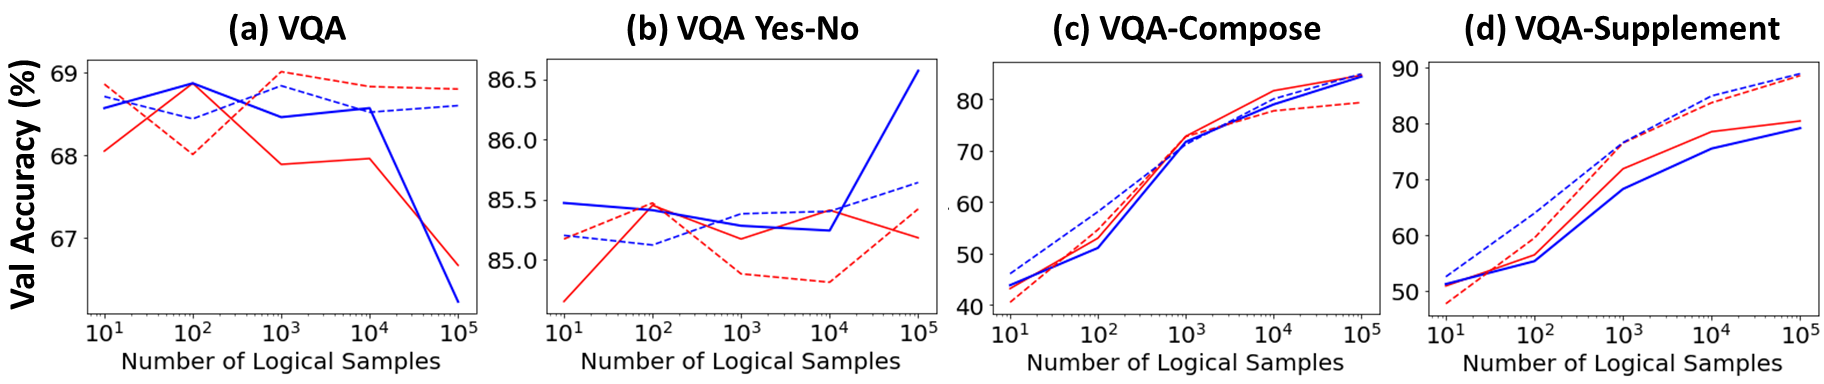
\includegraphics[width=\linewidth]{vqalol/images/fig_exp3_new.png}
    \caption{
    % Learning Curves: Red lines denote LXMERT, Blue lines denote our LOL model with $q_{\textit{ATT}}$. 
    % Models trained on VQA + \texttt{Comp} are shown in solid and those trained on VQA + \texttt{Comp} + \texttt{Supp} are in dotted lines. Best viewed in color.
    Learning Curve comparison for models (Red: LXMERT, Blue: LOL) trained on our datasets (solid lines: VQA~+~\texttt{Comp}, dotted lines: VQA~+~\texttt{Comp}~+~\texttt{Supp})
    }
    \label{fig:exp3}
\end{figure}


    \subsection{Can't We Just Parse the Question into Components?}
    
    Since our questions are a composition of multiple questions, an obvious approach is to split the question into its components, and to discern the logical formula for composition.
    The answers to these component questions (predicted by VQA models) can be \textit{re-combined} with the predicted logical formula to obtain the final answer.
    We use parsers to map components and logical operations to predefined slots in a logical function.
    The oracle parser uses the ground truth component questions and combines predicted answers using the true formula.
    However, at test time we do not have access to the true mapping and components.
    So we train a RoBERTa-Base~\citep{liu2019roberta} parser using B-I-O tagging~\citep{ramshaw-marcus-1995-text} for a Named-Entity Recognition task with constituent questions as entities.\footnotemark[1]
    
    The performance of the oracle parser serves as the upper bound as we have a perfect mapping, with the QA system being the only source of error.
    The trained parser has an exact-match accuracy of $85\%$, but only a $72\%$ accuracy in determining the number of operands.
    The parser has an accuracy of $89\%$ for questions with 3 or less operands, but only $78\%$ for longer compositions.
    End-to-end (E2E) models do not need to parse questions and hence overcome these hurdles, but do require an understanding of logical operations.
    Table~\ref{table:sota} shows that both oracle and trained parsers when used with LOL outperform parsers with LXMERT, by $6.82\%$) and $5.60\%$ respectively.
    The LOL model without using any parsers is better than both LXMERT and LOL with the trained parser by $7.55\%$ and $1.95\%$ respectively.

    \subsection{Explicit Training with Logically Composed Questions}
    \noindent\textbf{Can models trained on the VQA-v2 dataset answer logically composed questions?}
    The first section of Table~\ref{table:exp1} shows that LXMERT, when trained only on questions from VQA-v2 has near random accuracy ($\sim$50\%) on our logically composed datasets, thus exhibiting little robustness to such questions.\\
    
    \noindent\textbf{Can baseline model improve if trained explicitly with logically composed questions questions?}
    We train the models with data containing a combination of samples from VQA-v2, \texttt{VQA-Compose}, and \texttt{VQA-Supplement}.
    The accuracy on \texttt{VQA-Compose} and \texttt{VQA-Supplement} 
    improves, but there is a drop in performance on yes-no questions from VQA.
    Our models with our attention modules ($q_{\textit{\tiny ATT}}$ and $\ell_{\textit{\tiny ATT}}$) are able to retain performance on VQA-v2 while achieving improvements on all validation datasets.


    \subsection{Analysis}

        \noindent\textbf{Training with Closed Questions only:}
        We analyse the performance of models when trained only with closed questions from VQA, VQA + \texttt{Comp} and VQA + \texttt{Comp} + \texttt{Supp} and see that our model achieves the best accuracy on logically composed questions, as shown in sections 3 and 4 in Table~\ref{table:exp1}.
        Since we train only closed questions, we do not use our question attention module for this experiment.\\
        
        \noindent\textbf{Effect of Logically Composed Questions:}
        We increase the number of logical samples in the training data on a log scale from 10 to 100k.
        As can be seen from the learning curves in Figure~\ref{fig:exp3}(a), models trained on VQA + \texttt{Comp} + \texttt{Supp} are able to retain performance on VQA validation data, while those trained only on VQA + \texttt{Comp} data deteriorate.
        Figure~\ref{fig:exp3}(b) shows that our models improve on VQA Yes-No performance after being trained on more logically composed samples, exhibiting transfer learning capabilities.
        In (c) both our models are comparable to the baseline, but our model shows improvements over the baseline when trained on VQA + \texttt{Comp} + \texttt{Supp}.
        In (d) for all levels of additional logical questions, our model trained on VQA + \texttt{Comp} + \texttt{Supp} is the best performing.
        From (c) and (d), we observe that a large number of logical questions are needed during training for the models to learn to answer them during inference.
        We also see that our model yields the best performance on \texttt{VQA-Supplement}.\\
        
        \noindent\textbf{Compositional Generalization:}
        To test for compositional generalization, we train models on questions with a maximum of one connective (single) and test on those with multiple connectives.
        It can be seen from Table~\ref{table:exp4} that our models are better equipped than the baseline to generalize to multiple connectives and also to be able to generalize from \texttt{VQA-Compose} to \texttt{Supplement}.\\
        
            \begin{figure}
        \centering
            \subfloat[\label{heatmap_comp}]{%
            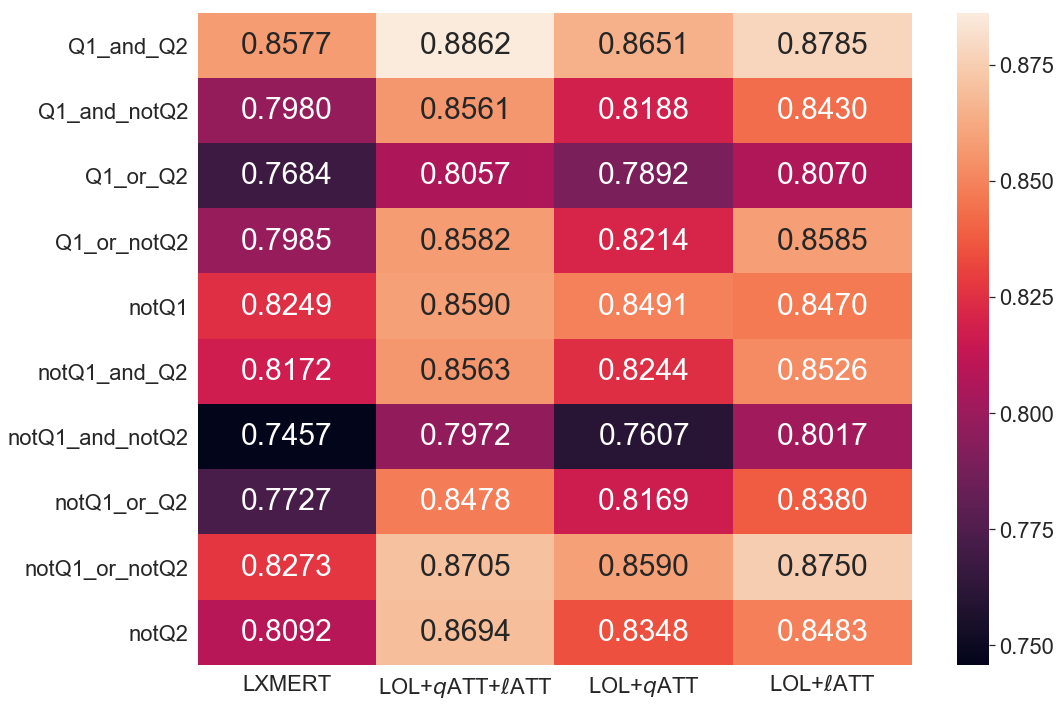
\includegraphics[angle=0,origin=c,width=0.6\linewidth]{vqalol/images/lol_heatmap.png}
            }\\
            \subfloat[\label{heatmap_supp}]{%
            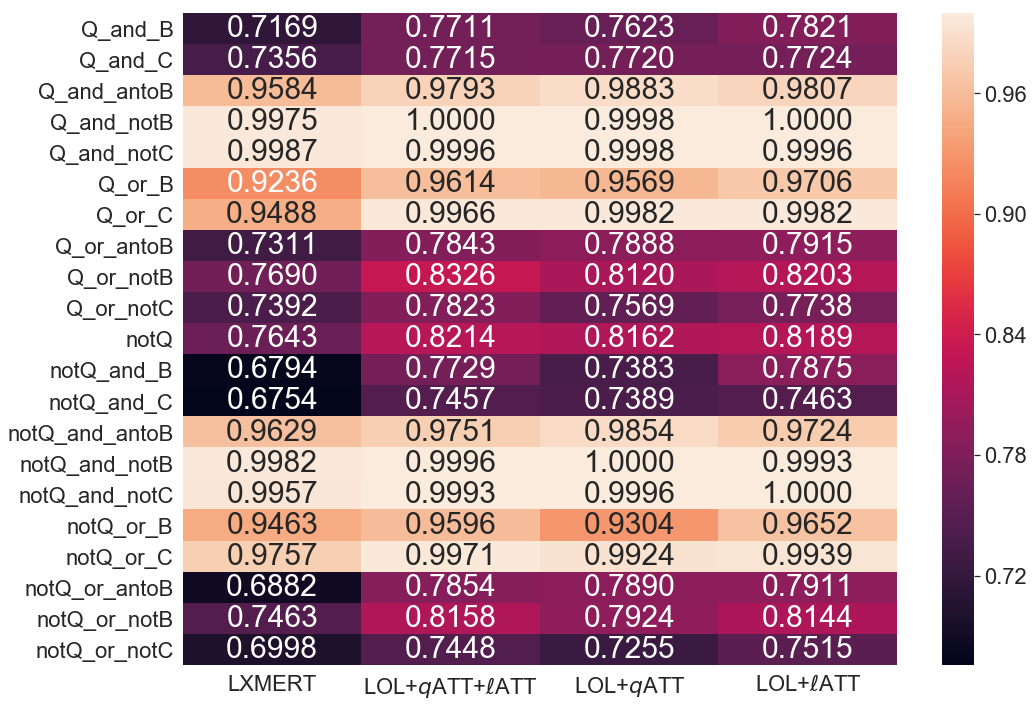
\includegraphics[angle=0,origin=c,width=0.65\linewidth]{vqalol/images/cwl_heatmap.png}
            }\\
            \subfloat[\label{varlen}]{%
            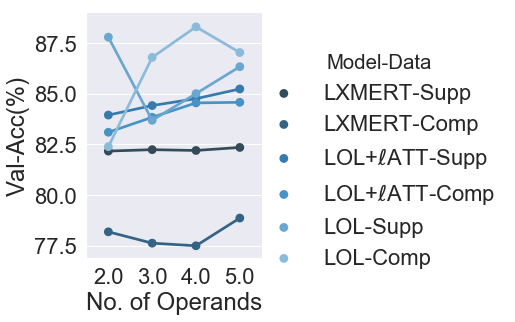
\includegraphics[angle=0,origin=c,width=0.4\linewidth]{vqalol/images/varlen_fixed2.png}
            }
        \caption{Accuracy for each type of question in (a) VQA-Compose, (b) VQA-Supplement and for questions with number of operands greater than 2.}
        \label{fig:heatmap}
    \end{figure}
        
        \noindent\textbf{Inductive Generalization:}
        We test our models on questions composed with more than two components. Parser-based  models have this property by default.
        As shown by Figure~\ref{varlen} our E2E models outperform the baseline LXMERT.\\

        \noindent\textbf{Commutative Property:}
        Our models have identical answers when the question is composed either as $Q_1\circ Q_2$ or $Q_2\circ Q_1$, for logical operation $\circ$, as shown in Table~\ref{table:exp4}.
        The parser-based models are agnostic to the order of components if the parsing is accurate, while our E2E models are robust to the order.\\

        \noindent\textbf{Accuracy per Category of Question Composition:}
        In Figure~\ref{fig:heatmap} we show a plot of accuracy versus question type for each model.
        $Q, Q_1, Q_2$ are questions from VQA, $B, C$ are object-based and caption-based questions from COCO respectively.
        From the results, we interpret that questions such as $Q\wedge antonym(B), Q\wedge\neg B, Q\wedge\neg C$ are easy because the model is able to understand absence of objects, therefore can always answer these questions with a ``NO".
        Similarly, $ Q\vee B, Q\vee C$ are easily answered since presence of the object makes the answer always ``YES".
        By simply understanding object presence many such questions can be answered. Figure~\ref{fig:heatmap} shows the model has the same accuracy for logically equivalent operations.

    \begin{table*}[t]
    \centering
     \resizebox{\linewidth}{!}{
    \begin{tabular}{@{}lllcccccccc@{}}
    \toprule
    \multirow{2}{*}{Model} & \multirow{2}{*}{Parser} & \multirow{2}{*}{\textbf{\pbox{20mm}{Training \\Data}}} & \multicolumn{4}{c}{\textbf{Test-Std. Accuracy (\%) $\uparrow$}} & \hphantom & \multicolumn{3}{c}{\textbf{Val. Accuracy (\%) $\uparrow$}}\\
     \cmidrule{4-7} \cmidrule{9-11}
     & & & Yes-No & Number & Other & Overall & & {Compose} & Supplement & Overall \\
    \midrule
    MCAN & None & VQA~\citep{Yu_2019_CVPR} & $86.82^{\#}$ & $53.26^{\#}$ & $60.72^{\#}$ & 70.90 & & 52.42 & {*} & {*}\\
    LXMERT & None & VQA~\citep{tan2019lxmert} & \textbf{88.20} & \textbf{54.20} & \textbf{63.10} & \textbf{72.50} & & 50.79 & 50.51 & 50.65\\
    LOL ($\mathit{q}$ATT) & None & VQA &  \underline{87.33} & \underline{54.03} & \underline{62.40} & \underline{72.03} & & 48.99 & 50.54 & 49.77\\
    \midrule
    LXMERT & Oracle & VQA & 88.20 & 54.20 & 63.10 & 72.50 & & 86.38 & 74.29 & 80.33 \\
    LXMERT & Trained & VQA & 88.20 & 54.20 & 63.10 & 72.50 & & 86.35 & 68.75 & 77.55\\
    LOL (full) & Oracle & VQA+Ours & 86.55 & 53.42 & 61.58 &71.04 & & 85.79 & 88.51 & 87.15\\
    LOL (full) & Trained & VQA+Ours & 86.55 & 53.42 & 61.58 &71.04 & & 82.13 & 84.17 & 83.15\\
    \midrule
    LXMERT & None & VQA+Ours & 85.23 & 51.25 & 60.58 & 69.78 & & 75.31 & 85.25 & 80.28 \\
    % LOL & None & VQA+Ours & 86.55 & 53.42 & 61.58 & 71.04 & & 72.88 & 88.32 \\
    LOL ($\mathit{q}$ATT) & None & VQA+Ours &  86.79 & 52.66 & 61.85 & 71.19 & & 79.88 & 87.12 & 83.50\\
    LOL (full)
    % ($\mathit{q}$ATT+$\ell$ATT) 
    & None & VQA+Ours & 86.55 & 53.42 & 61.58 &71.04 & & \underline{\textbf{82.39}} & \underline{\textbf{87.80}} & 85.10\\
    \bottomrule
    \end{tabular}
    }
    \caption[Test Set Results]{Performance on `test-standard' set of VQA-v2 and validation set of our datasets. LOL performance is close to SOTA on VQA-v2, but significantly better at logical robustness. $^*$\text{MCAN} uses a fixed vocabulary 
    % so we are unable to evaluate on 
    that prohibits evaluation on \texttt{VQA-Supplement} which has questions created from COCO captions. 
    $^{\#}$Test-dev scores, since MCAN does not report test-std single-model scores\footnotemark[2]}
    \label{table:sota}
\end{table*}
    \subsection{Evaluation on VQA v2.0 Test Data}
    Table~\ref{table:sota} shows the performance the VQA Test-Standard datset.
    Our models maintain overall performance on the VQA test dataset, and at the same time substantially improve from random performance ($\sim$ 50\%) on logically composed questions to 82.39\% on \texttt{VQA-Compose} and 87.80\% on \texttt{VQA-Supplement}.
    This shows that logical connectives in questions can be learned while not degrading the overall performance on the original VQA test set (our models are within $\sim$1.5\% of the state-of-the-art on all three types of questions on the VQA test-set).
    

%%%%%%%%%%%%%%%%%%%%%%%%%%%%%%%%%%%%%%%%%%%%%%%%%%%%%%%%%%%%%%%%%%%%%%%%%%%%%%%%
\section{Discussion}
%%%%%%%%%%%%%%%%%%%%%%%%%%%%%%%%%%%%%%%%%%%%%%%%%%%%%%%%%%%%%%%%%%%%%%%%%%%%%%%%
Consider the example, {\it ``Is every boy who is holding an apple or a banana, not wearing a hat?"}, humans are able to answer it to be true if and only if each boy who is holding \textit{at least one} of an apple or a banana is not wearing a hat~\citep{arlotti1263}.
Natural language contains such complex logical compositions, not to mention ambiguities and the influence of context.
In this paper, we focus on the simplest -- negation, conjunction, and disjunction.
We have shown that existing VQA models are not robust to questions composed with these logical connectives, even when we train parsers to split the question into its components.
When humans are faced with such questions, they may refrain from giving binary (Yes/No) answers.
For instance, logically, the question{\it ``Did you eat the pizza and did you like it?"} has a negative answer if either of the two component questions has a negative answer.
However, humans might answer the same question with the answer {\it ``Yes, but I did not like it"}.
While human question-answering is indeed elaborate, explanatory, and clarifying, that is the scope of our future work; here we focus only on predicting a single binary answer.

We have shown how connectives in a question can be identified by enhancing LXMERT encoders with dedicated attention modules and loss functions.
We would like to stress on the fact that we do not use knowledge of the connectives during inference, but instead train the network to be aware of it based on cross-modal features, instead of predicting purely based on language model embeddings which fail to capture these nuances.
% This work is an attempt to modularize the understanding of logical components to train the model to utilize the outputs of the attention modules.
We believe this work has potential implications on logic-guided data augmentation, logically robust question answering, and for conversational agents (with or without images).
Similar strategies and learning mechanisms will be used in the next chapter to operate ``logically'' in the image-space at the level of object classes and their attributes.


% \section{Conclusion}
% In this work, we investigate VQA in terms of logical robustness.
% The key hypothesis is that the ability to answer questions about an image, must be extendable to a logical composition of two such questions.
% We show that state-of-the-art models trained on VQA dataset lack this.
% Our solution involves the ``Lens of Logic" model architecture that learns to answer questions with negation, conjunction, and disjunction.
% We provide \texttt{VQA-Compose} and \texttt{VQA-Supplement}, two datasets containing logically composed questions to serve as benchmarks.
% Our models show improvements in terms of answering these questions, while at the same time retaining performance on the original VQA test-set.

% \section*{Acknowledgments}
% Support from NSF Robust Intelligence Program (1816039 and 1750082), DARPA (W911NF2020006) and ONR (N00014-20-1-2332) is gratefully acknowledged.